\documentclass[12pt,a5paper]{article}

\usepackage[T1]{fontenc} % font encoding, lubab õ tähte kasutada
\usepackage[utf8]{inputenc} % oleme siiski 21. sajandis, vajadusel on ka olemas utf8x
\usepackage{lmodern} % lmodern ja micrtype käivad käsikäes, teeb teksti ilusamaks
\usepackage{tikz}
\usetikzlibrary{decorations.pathreplacing, positioning}
\usepackage{microtype}
\usepackage[estonian]{babel} % eesti keele poolitamisreeglid jpm
\usepackage[per = fraction, expproduct=cdot, decimalsymbol=comma]{siunitx} % http://www.bakoma-tex.com/doc/latex/siunitx/siunitx.pdf
\usepackage{graphicx} 
\usepackage{wrapfig}
\usepackage{epstopdf} %minul on vaja, et .eps pilte saada
\usepackage{icomma} %koma arvust mõistlikul kaugusel
\usepackage{amsmath}
\usepackage{enumitem}
\usepackage{caption}
\usepackage{pgfplots}
\usepackage{float}

\special{papersize=14.85cm,21cm}

%paneme kõik mõõdud paika
\topmargin=-2.5cm \textheight=18.5cm \textwidth=12.77cm
\oddsidemargin=-1.5cm  \evensidemargin=-1.5cm
\setlength{\parindent}{0pt} \setlength{\parskip}{6pt} \sloppy

\relpenalty=10000 \binoppenalty=10000 % Tekstisisestes valemites reavahetusi ärgu olgu


\pagestyle{empty} % ilma leheküljenumbrita

\newcommand{\numb}[1]{\vspace{5pt}\textbf{\large #1}}
\newcommand{\nimi}[1]{(\textsl{\small #1})}
\newcommand{\punktid}[1]{(\emph{#1~p.})}
\newcounter{ylesanne}
\newcommand{\yl}[1]{\addtocounter{ylesanne}{1}\numb{\theylesanne.} \nimi{\bf{#1}} \newblock{}}
\newcommand{\pp}[1]{[\textbf{#1~p.}]}
\newcommand{\pv}[1]{\quad \hbox{[\textbf{#1~p.}]}}
\newcommand{\ue}[1]{\underline{\emph{#1}}}
\newcommand{\hence}{\quad \Rightarrow \quad}
\newcommand{\autor}[1]{\emph{ Autor: #1.\\}}
\newcommand{\lautor}[1]{\emph{ Lahenduse autor: #1.\\}}

\makeatletter
\newcommand*\bigcdot{\mathpalette\bigcdot@{.8}}
\newcommand*\bigcdot@[2]{\mathbin{\vcenter{\hbox{\scalebox{#2}{$\m@th#1\bullet$}}}}}
\makeatother

\begin{document}

\begin{center}
\textbf{\Large Eesti koolinoorte 67. füüsikaolümpiaad} \vspace{2pt}

\emph{18. jaanuar 2020. a. Piirkondlik voor.}

\emph{{\bf Gümnaasiumi} ülesannete lahendused}


\end{center}

\numb{Eessõna}

Allpool on toodud iga ülesande üks õige lahenduskäik (mõnel juhul ka
enam). \textbf{Kõik alternatiivsed õiged lahenduskäigud tuleb hinnata samuti maksimumhindega.} Iga alternatiivse lahenduskäigu jaoks tuleb
kontrollijatel koostada hindamisskeem, juhindudes võimalusel juuresoleva
hindamisskeemi punktijagamisproportsioonist. Soovituslikud
maha-arvamise punktid: numbriline arvutusviga --- 0,5; viga
teisendustes --- 0,5 p. (märgi jms väiksem viga) või 1 p. (viga, mis
viib dimensioonide konf\/liktini), maha arvata ainult üks kord, st
edasikanduvat viga mitte karistada; kui vastus tuleb füüsikaliselt
absurdne, siis võib täiendavalt karistada 0,5 punktiga; üksik viga
lähtevalemis: 0,5 p. (kui märgiviga), kuni 50\% (sisuline viga).


\yl{SAUN} \punktid{6} \autor{Richard Luhtaru}
Vee mass on $m=\rho V$ ja seega vee soojendamiseks ja aurustumiseks kuluv soojushulk on
$$Q=c_v\rho V (T_k-T_0) + L\rho V, \qquad\pp{1}$$
kus $T_k = \SI{100}{\celsius}$ on keemistemperatuur ja $T_0$ on vee algtemperatuur.

Kui kerise temperatuur väheneb $\Delta T$ võrra ($\Delta T$ on temperatuuri muutuse absoluutväärtus), siis kerise poolt antud soojushulk on
$$Q=c_kM\Delta T \qquad \pp{1}$$
Võrdustades seosed saame
$$\Delta T = \frac{\rho V\left(c_v(T_k-T_0)+L\right)}{c_kM} \qquad\pp{1}$$
Asendades sisse antud väärtused, saame
$$\Delta T_{\text{(külm)}}\approx \SI{7.65}{\celsius} \qquad\pp{1}$$
$$\Delta T_{\text{(kuum)}}\approx \SI{6.81}{\celsius} \qquad\pp{1}$$
Kuna $\frac{\num{7.65}-\num{6.81}}{\num{6.81}}\approx \num{0.12}$ \pp{0,5} on suurem kui 10\%, siis Juhanil ei ole õigus. \pp{0,5}

\emph{Märkus.} Viimases reas lugeda õigeks ka lahendus, mis leiab $\frac{\num{7.65}-\num{6.81}}{\num{6.81}}$ asemel $\frac{\num{7.65}-\num{6.81}}{\num{7.65}}$ väärtuse või leiab, et $\frac{\num{7.65}}{\num{6.81}}>\num{1.1}$.


\yl{KARUSSELL} \punktid{8} \autor{Krister Kasemaa}
Karuselli ketid on pinge all, olgu kettide pinge $T$. Pinget $T$ saab jagada $x$ ja $y$ komponentieks: \pp{1} 
$$T_x=T \cdot \sin{\theta}$$
$$T_y=T \cdot \cos{\theta} \qquad \pp{1} $$
 \begin{center}
\includegraphics[width=0.3\textwidth]{Karussell}
\end{center}
Ketid on horisontaaltasandis ringliikumses, olgu selle joonkiirus $v$. Seega võrdub pinge horisontaalsunnaine projektsioon tsentrifugaaljõuga:
$$T_x = \frac{m v^2}{R_{p}}\quad\quad \pp{1}$$
kus $m$ on Juku mass ja $R_{p} = R + l \cdot \sin{\theta}$ on pöörlemisraadius.
\\
Vertikaalteljes on jõud tasakaalus:
$$T_y=mg \quad \quad \pp{1}$$ 
\\
Asendades $T_x$ ja $T_y$ asemele $T \cdot \sin{\theta}$ ja $T \cdot \cos{\theta}$ ning $R_{p}$, saame võrrandisüsteemi:
$$T \cdot \sin{\theta} = \frac{m v^2}{R + l \cdot \sin{\theta}}$$
$$T \cdot \cos{\theta} = mg \qquad \pp{1}$$ 
\\
Jagades esimese võrrandi teisegas
$$\tan{\theta}= \frac{mv^2}{g(R + l \cdot \sin{\theta})}$$
avaldub lõbusõitja joonkiirus:
$$v= \sqrt{g \cdot \tan{\theta} \cdot (R + l \cdot \sin{\theta})}\approx \SI{14.1}{m/s}. \qquad \pp{1}$$ 
\\
Selleks et leida pöörete arvu minutis, leiame esmalt ühe pöörde aja, ehk perioodi $T$:
$$T=\frac{2 \pi R_{p}}{v}=\frac{2 \pi (R + l \cdot \sin{\theta})}{v}. \qquad \pp{1}$$ 
\\
Seega pöörete arv  $\Delta t = 60\;$s jooksul on
$$N=\frac{\Delta t}{T} =\frac{\Delta t \cdot v}{2 \pi (R + l \cdot \sin{\theta})} \approx \SI{11.5}{}. \qquad \pp{1}$$ 



\yl{HÜPPAV SILINDER} \punktid{8} \autor{Päivo Simson}

\emph{Lahendus 1.}
Vaatleme kõigepealt silindri liikumist energiakadu arvestamata. Olgu silindri veest väljumise kõrgus $x$. Silindri potentsiaalne energia kasvab liikumise käigus
\[
\Delta U_s=mg(h+x)\quad[\textbf{1 p.}]
\]
võrra. See muutus on võrdne üleslükkejõu tööga, mida saab arvutada kui tööd, mida tuleb teha silindri poolt välja tõrjutud vee tõstmiseks pinnale. Välja tõrjutava vee mass $m_v=\pi r^2 h \rho_v$ ja selle massikese asub sügavusel $h/2$. Üleslükkejõu töö on seega
\[
A=m_v\frac{h}{2}=\pi r^2 h \rho_v\frac{h}{2}.\quad[\textbf{4 p.}]
\]
Võrdusest $\Delta U_s=A$ saame
\[
x=h\left(\frac{\pi r^2 \rho_v h}{2m}-1\right) \quad[\textbf{2 p.}]
\]
Et pool kineetilisest energiast läheb veest väljumisel kaduma, siis on tegelik kõrgus $H$ saadud väärtusest poole väiksem
\[
H=\frac{x}{2}\approx\SI{40.0}{cm}. \quad[\textbf{1 p.}]
\]


\emph{Lahendus 2.}

Olgu $x$-telg suunatud vertikaalselt üles ja nullpunkt asugu veepinnal. Vaatleme kõige\-pealt silindri alumise otsa liikumist vahemikus $x=-h...0$ ja leiame silindri kineetilise energia veest väljumise hetkel. Silindrile mõjub
gravitatsioonijõud ${F_g=-mg}$ ja üleslükkejõud $F_\text{\emph{\"u}},$ mis kõrgusel $x$ avaldub kujul $F_\text{\emph{\"u}}=g\rho_vV=-g\rho_v \pi r^2 x$, [\textbf{2 p.}] kus $V$ on silindri veealuse osa ruumala ($x$-koordinaat on vaadeldavas piirkonnas negatiiv\-ne). Näeme, et üleslükkejõud toimib analoogselt vedru elastsusjõuga $F_e=-kx$, mille potentsiaalne energia avaldub kujul $U_e=\frac{1}{2}kx^2$. Üleslükkejõule vastab antud juhul järelikult potentsiaalne energia $U_\text{\emph{\"u}}=\frac{1}{2}g\rho_v \pi r^2 x^2$. Silindri koguenergia on seega
\[
	E=\frac{mv^2}{2}+mgx+\frac{1}{2}g\rho_v \pi r^2 x^2. \quad[\textbf{2 p.}]
\]
Kui $x=-h$, siis $v=0$ ja koguenergia väärtus on järelikult
\[
	E=\frac{1}{2}g\rho_v \pi r^2 h^2-mgh. \quad[\textbf{1 p.}]
\]
Et pool sellest läheb teksti kohaselt kaduma, siis on pärast veest väljumist koguenergia väärtus $E/2$ ja silindri kineetiline energia
\[
	\frac{mv_0^2}{2}=\frac{1}{4}g\rho_v \pi r^2 h^2-\frac{1}{2}mgh. \quad[\textbf{1 p.}]
\]
Edasi toimub silindri liikumine vastavalt kinemaatika valemitele $x=v_0t-gt^2/2$ ja $v=v_0-gt$. Et trajektoori kõrgeimas punktis $v=0$, siis saame teisest kinemaatika võrrandist $t_{max}=v_0/g$, mis vastab hetkele, mil silinder on maksimaalsel kõrgusel. Maksimaalne kõrgus on järelikult
\[
	H=v_0t_{max}-gt_{max}^2/2=\frac{v_0^2}{2g}=\frac{h}{2}\left(\frac{\pi r^2\rho_v h}{2m}-1\right)\approx \SI{40.0}{cm}. \quad[\textbf{2 p.}]
\]


\begin{wrapfigure}{r}{0.3\textwidth}
    \vspace{-30pt}
	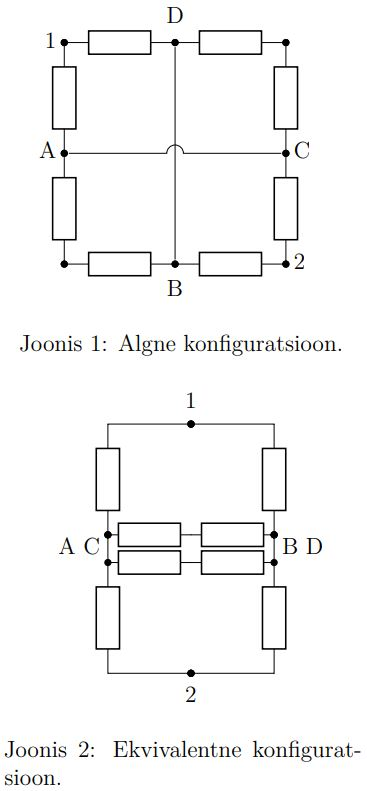
\includegraphics[width=0.28\textwidth]{ruut_lah.jpg}
	\vspace{-40pt}
\end{wrapfigure}
\yl{ELEKTRIRUUT} \punktid{8} \autor{Sandra Schumann}
Tähistame joonisel punktid A, B, C
ja D. Paneme tähele, et kuna
A ja C on ühendatud omavahel
juhtmega, mille takistuse võime
lugeda nulliks, siis A = C \pp{1}. Samal
põhjusel B = D \pp{1}. Nüüd võime
skeemi ümber joonistada nii, nagu
näidatud joonisel 2. \pp{2}

Sümmeetria tõttu ei läbi punktide A, C ja B, D vahelist silda kunagi vool \pp{2}, seega lihtsustub skeem
kujule, kus on vaid neli ülejäänud takistit \pp{1}, mille kogutakistuseks tuleb $\frac{2R}{2} = R$ \pp{1}

\yl{PURILENNUK} \punktid{8} \autor{Andreas Valdmann}
\begin{center}
	\vspace{-30pt}
  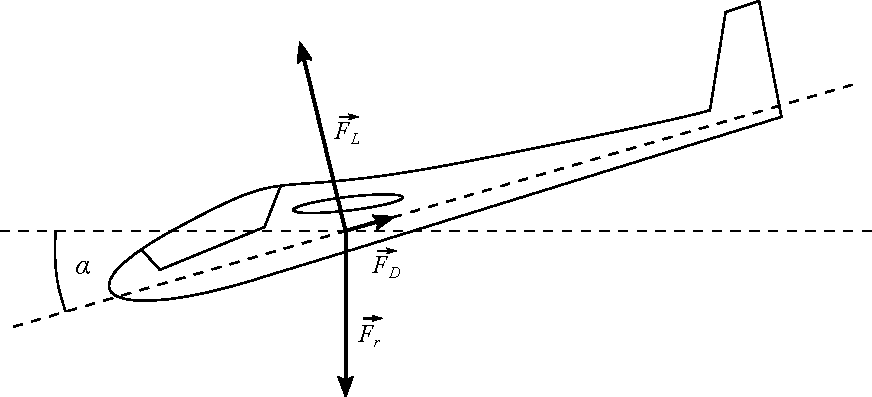
\includegraphics[width=0.7\textwidth]{purilennuk_joonis.pdf}
\end{center}


Vaatleme purilennukile mõjuvaid jõude pukseerimise ajal ja vabal liuglemisel. Pukseerimise ajal mõjuvad purilennukile horisontaalselt puksiirköie tõmbejõud $T$ ning õhutakistus $F_D$ ja vertikaalselt raskusjõud $F_r = mg$ ning aerodünaamiline tõstejõud $F_L$. Ühtlase kiirusega lendamisel on purilennukile mõjuvate jõudude (vektoriaalne) summa 0, millest $F_D = T$ ja $F_L = mg$. Seega on purilennuki aerodünaamilisi omadusi iseloomustav suhe antud juhul avaldatav kui
\begin{equation}
	\frac{F_L}{F_D} = \frac{mg}{T}.
\end{equation}

Vabal liuglemisel moodustab lennuki kiirusvektor horisontaalsihi suhtes nurga $\alpha$ ja antud olukorras lennukile mõjuvad jõud on kujutatud joonisel.


Kuna lennuki kiirus on ka sel juhul ühtlane, siis peab jällegi kehtima jõudude tasakaal ehk kõigi kolme jõu vektoriaalne summa on 0. Jõudude horisontaalkomponentide tasakaalust saame $F_L\sin(\alpha) = F_D\cos(\alpha)$, millest:
\begin{equation}
	\frac{F_D}{F_L} = \frac{\sin(\alpha)}{\cos(\alpha)}=\tan(\alpha).
\end{equation}
Märkus: jõudude $F_L$ ja $F_D$ absoluttväärtused on pukseerimisel ja liuglemisel mõnevõrra erinevad, kuid nende suhe $F_D/F_L$ on mõlemal juhul sama.
Viimaks paneme tähele, et kuna purilennuki kiirusvektor moodustab horisontaalsihiga nurga $\alpha$, siis saame maksimaalse lennukauguse $s$ leida täisnurksest kolmnurgast kaatetitega $s$ ja $h$ ning alusnurgaga $\alpha$ ehk $h/s = \tan{\alpha}$. Eelnevalt leitud seoseid kasutades saame
\begin{equation}
s = \frac{h}{\tan(\alpha)} = \frac{hF_L}{F_D} = \frac{hmg}{T},
\end{equation}
mille arvväärtus on $s = \SI{82}{km}$.



\yl{KELL} \punktid{10} \autor{Kaur Aare Saar}
Leiame kummagi osuti jaoks maksimaalse võimsuse, mis nende liigutamiseks saab
kuluda. See juhtub siis, kui vastav seier on $9$ peal, sest tööd tuleb teha
gravitatsioonijõu vastu ja konstanse kiiruse korral on vajaminev jõud suurim
siis kui jõud mille vastu tööd tehakse on antiparalleelne masskeskme
kiirusvektoriga.
$$P_{max} = F v = mg \frac{2 \pi \frac{L}{2}}{T} = \frac{\pi mgL}{T},$$
kus $T$ on vastava seieri täispöörde tegemiseks kuluv aeg.
Minutiosuti jaoks on vastav periood $T_1={60\cdot60}$ s ning võimsus $P_1 =\SI{6.41}{\micro\watt}$.
Tunniosuti jaoks on vastav periood $T_2={12\cdot 60\cdot60}$ s ning võimsus $P_2=\SI{1.78}{\micro\watt}$. Seega summaarselt saaks
seierite liigutamine võtta võimsust $P_1+P_2 = \SI {8.20}{\micro\watt}$.
Vooluallikas suudab seiereid liigutada kasuliku võimsusega
$P=\eta VI=\SI{1.5}{\milli\watt}$. See on aga rohkem kui osutite liigutamiseks
vaja läheb, seega kell ei jää seisma.

\textbf{Vastus:}
Kell ei jää seisma, kuniks kella vooluallikas annab voolu vähemalt
$\SI {8.20}{\micro\watt}$.


\yl{JÄLLE SAUNA!} \punktid{10} \autor{Jaan Kalda}
Vesi keeb 100 kraadi juures ja tekkinud veeaur kaotab hea soojusliku kontakti kerisekividega ning seetõttu ei jõua oluliselt üle 100 kraadi kuumeneda. \pp{2} Niisiis võime eeldada, et $\nu_a=p_0V/RT_a\approx 341$ mooli õhku \pp{1} temperatuuril $T_a$ seguneb $\nu_w=m/\mu_w\approx 11$ mooli veeauruga \pp{1} temperatuuril $T_a+\Delta T$, kus $\Delta T=\SI {20}\celsius$ \pp{1}. Seega saame soojusbalansi kirja panna kujul $c_{pw}\nu_w(\Delta T-\delta T)=c_{pa}\nu_a\delta T$ \pp{2}, kus $\delta T$ tähistab õhutemperatuuri muutu ja $c_{pa}=c_a+R$ \pp{1} ning $c_{pw}=c_w+R$ \pp{1} tähistavad õhu ja veeauru molaarseid erisoojusi konstantsel rõhul. (Kasutada tuleb erisoojust konstantsel rõhul, sest kogu protsess toimub konstantse atmosfäärirõhu juures --- üleliigne õhk pääseb välja; kes kasutab $c_a$-d ja $c_w$-d jääb neist kahest punktist ilma.) Siit saame $\delta T=c_{pw}\nu_w\Delta/(c_{pw}\nu_w+c_{pa}\nu_a)\approx\SI{0.3}\celsius$ \pp{1}. Nagu näeme on temperatuuri muutus üsna väike, subjektiivselt hakkab palavam õhuniiskuse tõusu tõttu. Pikemas ajaskaalas leil jahutab kerisekive, mis ei kuumuta enam õhku endise võimsusega ja temperatuur võib hoopis langema hakata.


\yl{DIOODID} \punktid{10} \autor{Jaan Kalda}
Lahendus: Kuivõrd dioodid on ühendatud paralleelselt, siis nende pinged on võrdsed  \pp{2}. Ilmselt kõige lihtsam moodus on katse-eksituse meetodil sellise pinge $V_0$ leidmine, mille korral dioodide voolude summa on võrdne $I_0$-ga, $I_1(V_0)+I_2(V_0)=I_0$  \pp{2}. Otsime lahendit piirkonnas, kus keskmine vool on pool vooluallika voolust, st 1.35 amprit  \pp{1}; seal piirkonnas on pinge umbes $V_0\approx \SI{3.6}V$ \pp{1} ja fikseeritud pinge $V_0$ juures on kahe voolutugevuse vahe $\Delta I = \SI {0.20}A$  \pp{1}. Seega $I_1=\SI{1.25}A$ [\pp{0.5} väärtuse eest, mis on vahemikus $\SI{1.22}A$ kuni $\SI{1.28}A$  ja rahuldab tingimust $I_1(V_0)+I_2(V_0)=\SI{2.7}A$] ning $I_2=\SI{1.45}A$ [\pp{0.5} väärtuse eest, mis on vahemikus $\SI{1.42}A$ kuni $\SI{1.48}A$ ja rahuldab tingimust $I_1(V_0)+I_2(V_0)=\SI{2.7}A$]. (Kui voolude väärtused on etteantud vahemikus, kuid summa erineb 2.7 amprist, siis arvväärtuste eest punkte ei saa.) Kuivõrd dioodide pinged on samad, siis võimsuste suhe on voolude suhe, st võimsuste suhteline erinevus on $2\Delta I/I_0\approx 15$\%  (\pp{1} avaldise ja \pp{1} väärtuse eest; kui lõppvastus on vahemikus 13\% kuni 18\%, siis antakse väärtuse eest täispunktid; kui lõppvastus on väiksem 10\%-st või suurem 22\%-st, siis arvväärtuse punkte ei anta; ülejäänud juhtumeil antakse 0.5 punkti). Märkus: aktsepteeritavad on kõik lähenemised, mis jõuavad õige tulemuseni $I_1$ ja $I_2$ jaoks tuginedes lahenduse alguses toodud kahele tingimusele pingete ja voolude jaoks.

\vspace{10pt}
\yl{LAENGUD MAGNETVÄLJAS} \punktid{12} \autor{Jaan Kalda}
\vspace{-10pt}
  \begin{center}
    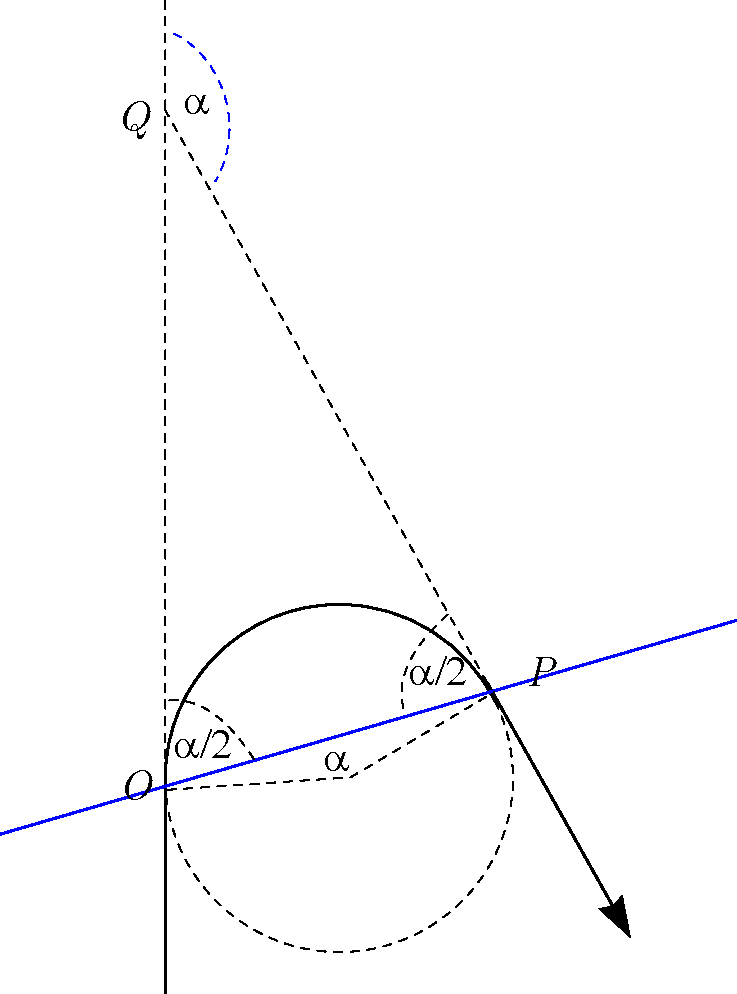
\includegraphics[width=0.5\textwidth]{laeng_b-s}
  \end{center}
  \vspace{-10pt}
Lahendus. Sisenegu osake punktis $O$ ja väljugu punktis $P$, kusjuures punkte $O$ ja $P$ ühendab ringjoone kaar --- osakese trajektoor magnetväljas. Lõikugu osakese trajetoori sirgjooneliste lõikude pikendused punktis $Q$, vt joonis. Ülesande tingimuse kohaselt on nurk sirgete $OQ$ ja $QP$ vahel $\alpha$. Et kolmnurk $OQP$ on sümmeetria tõttu võrdhaarne, siis $\angle OQP=\alpha/2$  \pp{3}. Seega peab punkt $P$ asuma sõltumata ringjoone raadiusest sirgel $OP$, mis on $y$-telje suhtes nurga $\alpha/2$ all  \pp{2}, st $f(x)=x\cot(\alpha/2)$  \pp{1}. Punktid joonise eest: on näidatud vähemalt üks trajektoor, millel on kaks sirgjoonelist segmenti, mis on üksteise suhtes nurga $\alpha$ all --- trajektoori osad enne ja pärast magneväljas viibimist --- \pp{2} (kui joonis käsitleb vaid erijuhtu $\alpha=180^\circ$, siis ainult \pp{1}); neid segmente ühendab ringjoone kaare kujuline segment --- \pp{2}; üleminek sirgjooneliselt trajektoorilt ringjooneliseks ja vastupidi on ilma murdekohata (st sirge on ringjoone puutujaks) --- \pp{2}.

\vspace{10pt}
\yl{TELESKOOP} \punktid{12} \autor{Eero Uustalu}
Kui koostaksime teleskoobi vaid kahest komponendist siis nurksuurenduse saamiseks peame eelkõige tekitama olukorra kus optiliste komponentide fookuskaugused on erinevad.
Kõrvuti asetatud õhukeste läätsede optilised tugevused liituvad. Kahe läätse liitmisel saame seega läätse fookuskaugusega $ \frac{f}{2} $ ja kui asetaksime kolm läätse kõrvuti siis ühendläätse fookuskauguseks kujuneks $ \frac{f}{3} $

\vspace{20pt}
\emph{Variant 1}\\
\textbf{Teleskoop mis koosneks siis ühest üksikust läätsest ja ühest kaheläätselisest komponendist annaks suurenduse 2 korda.}

\vspace{-10pt}
  \begin{center}
    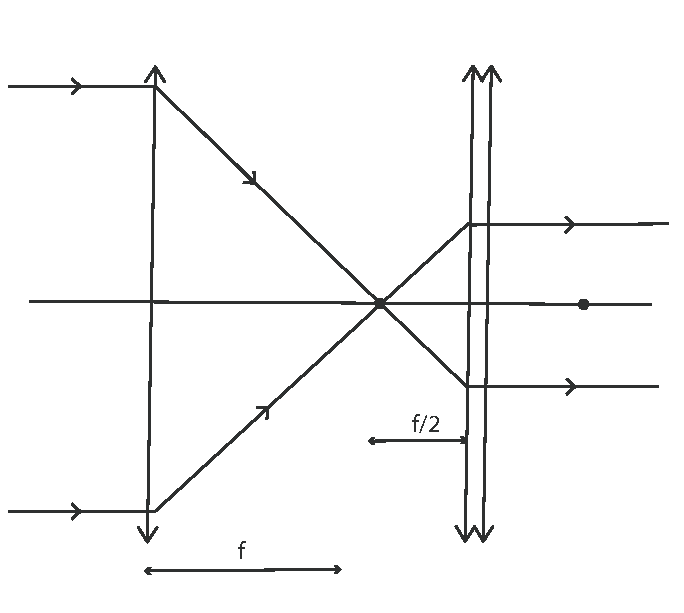
\includegraphics[width=0.45\textwidth]{laatsed_lah1}
  \end{center}
  \vspace{-10pt}
  


\emph{Variant 2}\\
\textbf{Teleskoop mis oleks koostatud ühest üksikut läätsest ja ühest kolmeläätselisest komponendist annaks suurenduse 3 korda.}

\vspace{-10pt}
  \begin{center}
    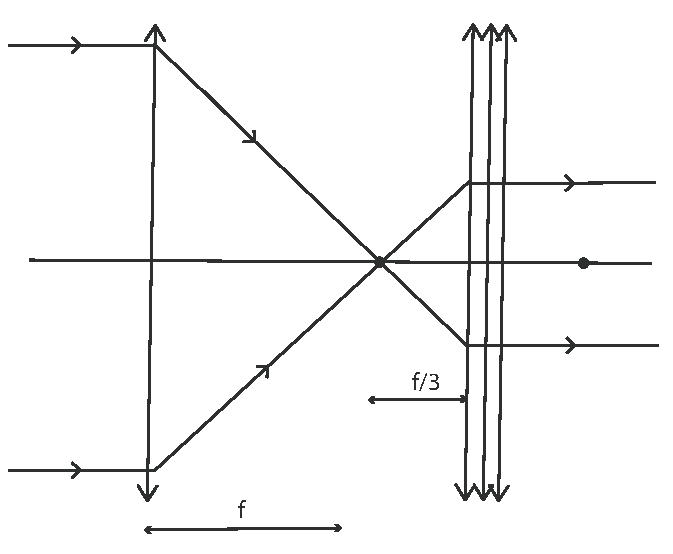
\includegraphics[width=0.45\textwidth]{laatsed_lah2}
  \end{center}
  \vspace{-10pt}


\emph{Variant 3}\\
\textbf{Suurema suurenduse saaks aga hoopis kolmekomponendilise  või neljakomponendilise skeemiga.}

Vaaltleme kahte skeemi:

\textbf{kolm lihtläätse järjest}

\vspace{-10pt}
  \begin{center}
    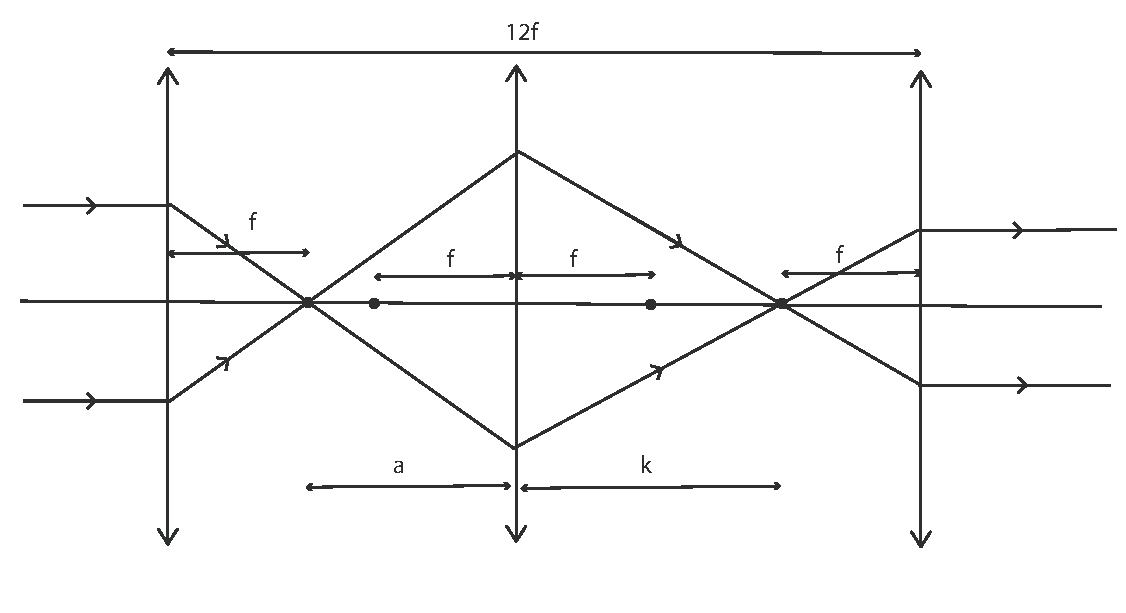
\includegraphics[width=0.8\textwidth]{laatsed_lah4}
  \end{center}
  \vspace{-10pt}

\textbf{lihtlääts - kaheläätseline liitlääts - lihtlääts}

\vspace{-10pt}
  \begin{center}
    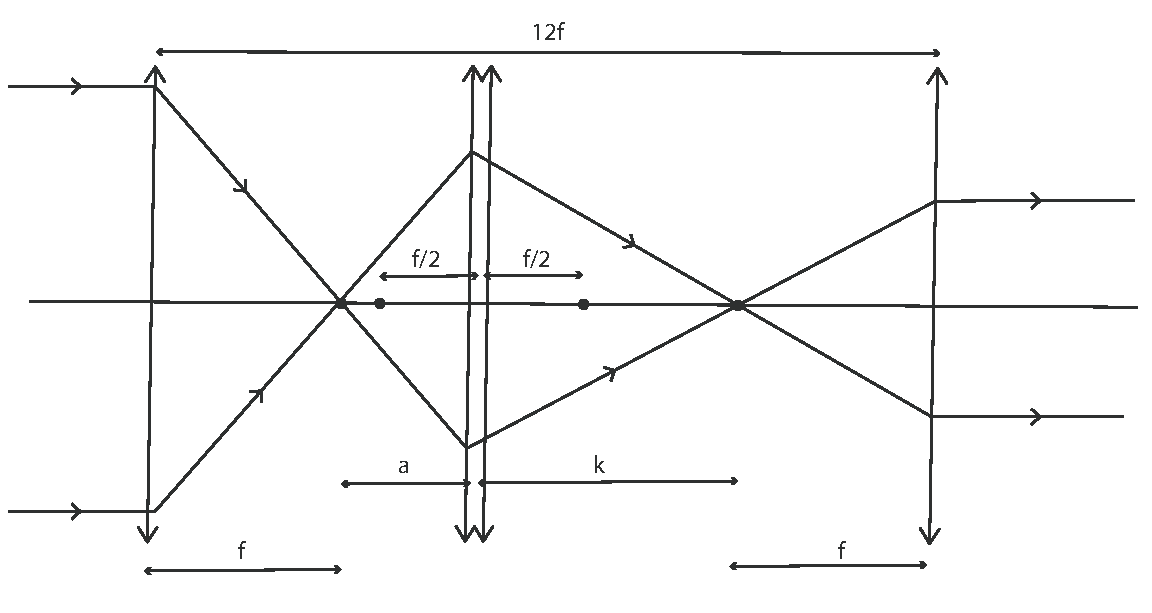
\includegraphics[width=0.8\textwidth]{laatsed_lah3}
  \end{center}
  \vspace{-10pt}

Nimelt hakkab keskmine lääts sellise skeemi korral käituma justkui kaks kõrvutiasetatud läätse fookuskaugustega vastavalt $ a $ ja $ k $ .

Süsteemi kogusuurenduseks tuleks sel juhul

 $ {\beta}_{kogu} = {\beta}_1 \cdot {\beta}_2 = \frac {f} {a} \cdot \frac {k} {f} = \frac {k}{a}$

Näeme et parima tulemuse saame kui $a$ oleks võimalikult väike ja $k$ oleks võimalikult suur.

Üheläätselise keskläätse puhul ei saa  $a$ olla väiksem kui $f$ (on sellest natukene suurem).

Kaheläätselise keskläätse puhul ei saa aga $a$ olla väiksem kui $ \frac {f}{2}$ (on sellest natukene suurem).

Samas aga $k$ väärtust piirab vaid süsteemi kogupikkusest tulenev piirang. See on aga mõlema süsteemi jaoks ühesugune (tõsi, kaheläätselise keskkomponendi puhul on sama üldpikkuse korral $k$ $ \frac{f}{2}$ võrra pikem) ning tulenevalt suurenduse valemist annab  suurima suurenduse just kaheläätselise keskkomponendiga süsteem!

\textbf{Seega} asetame üksikläätsed toru otstesse ja topeltläätse esiläätsele võimalikult lähedale nii, et esimese läätse fookuse kujutis tekiks kaksikläätse abil tagumise läätse fookusesse.
Kaheläätselise keskelemendiga süsteemi jaoks saame seosed

$ 12f = f + a + k + f $ ehk $ 10f = a + k $ ehk $ k = 10f - a $

ja

$ \frac{2}{f} = \frac{1}{a} + \frac{1}{k} $

asendame esimese teise

$ \frac {2}{f} = \frac {1}{a} + \frac {1}{10f - a} $

viime ühisele nimetajale, ristkorrutis, jagame miinus kahega, saame ruutvõrrandi

$ a^2 - 10fa + 5f^2 =0 $

mille lahendiks on $ a = (5 \pm \sqrt{20}) f $ kust $a=0.52786f $ ja $k=9.47213f$ .

Maksimaalseks suurenduseks tuleb seega $ {\beta}_{kogu} = 17.944 \approx 18 $ .


\emph{Variant 4}\\
\textbf {Kui kolmekomponendilises süsteemis kasutati siiski vaid üheläätselist keskelementi saame seosed:}

$ 12f = f + a + k + f $ ehk $ 10f = a + k $ ehk $ k = 10f - a $

ja

$ \frac {1}{f} = \frac{1}{a} + \frac{1}{k} $

asendame esimese teise

$ \frac {1}{f} = \frac {1}{a} + \frac {1}{10f - a} $

viime ühisele nimetajale, ristkorrutis, saame ruutvõrrandi

$ a^2 - 10fa + 10f^2 =0 $

mille lahendiks on $ a = (5 \pm \sqrt{15}) f $ kust $a=1.12702f $ ja $k=8.87298f$ .

Maksimaalseks suurenduseks tuleb seega $ {\beta}_{kogu} = 7.872 \approx 8 $ .

\emph{Variant 5}\\
\textbf {Üks variantidest on ka nelja läätsega süsteem:}

Puudusesks on nagu ka kolmest lihtläätsest süsteemi korral sama suurenduse saamiseks vajalik suurem üldpikkus.

\vspace{-10pt}
  \begin{center}
    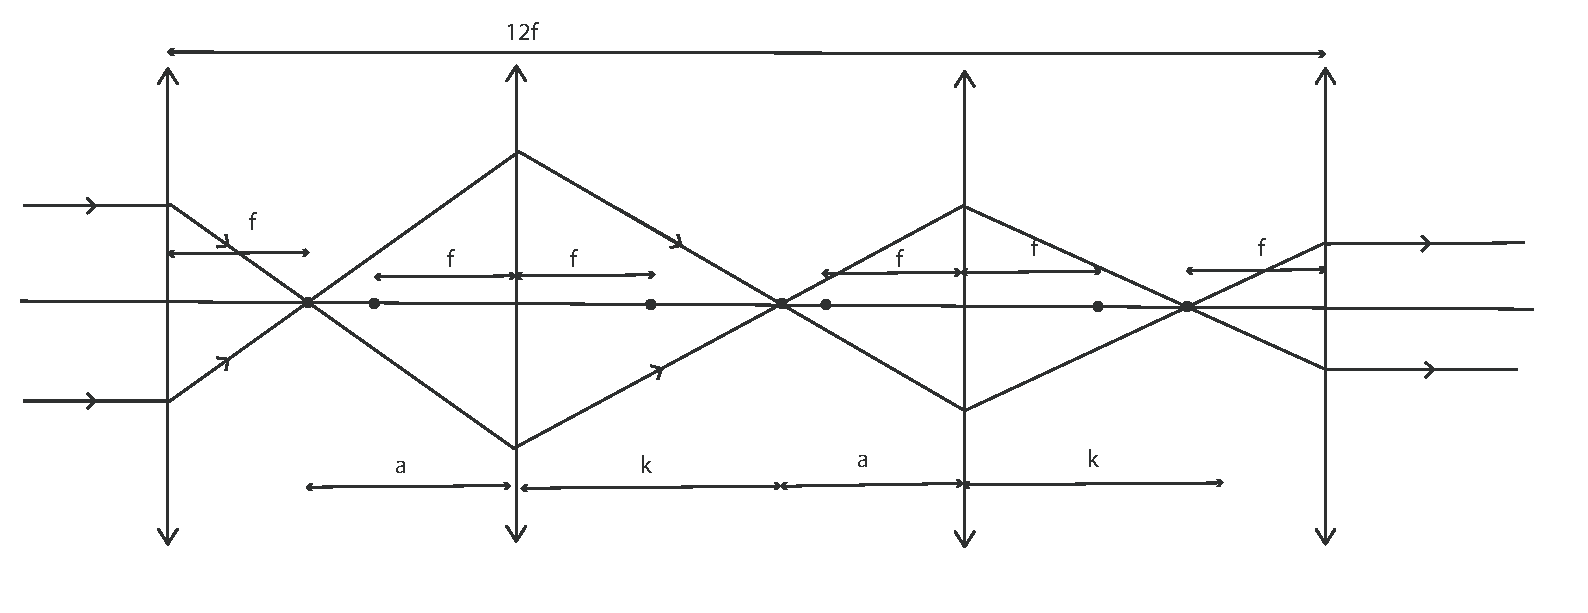
\includegraphics[width=1\textwidth]{laatsed_lah5}
  \end{center}
  \vspace{-10pt}


$ 12f = f + a + k + a + f $ ehk $ 5f = a + k $ ehk $ k = 5f - a $

ja

$ \frac {1}{f} = \frac{1}{a} + \frac{1}{k} $

asendame esimese teise

$ \frac{1}{f} = \frac {1}{a} + \frac{1}{5f - a} $

viime ühisele nimetajale, ristkorrutis, saame ruutvõrrandi

$ a^2 - 5fa + 5f^2 =0 $

mille lahendiks on $ a = (2.5 \pm \sqrt{1,25}) f $ kust $a=1.38197f $ ja $k=3.61803f$ .

Maksimaalseks suurenduseks tuleb seekord aga  
\[ {\beta}_{kogu} = {\beta}_1 \cdot {\beta}_2 \cdot {\beta}_3 = \frac {f}{a} \cdot \frac {k}{a} \cdot \frac {k}{f} = {(\frac {k}{a})}^2 = 2.618^2 = 6.854 \approx 7. \]

\end{document}

